\documentclass[tikz,border=4pt]{standalone}
\usepackage{amsmath}
\begin{document}
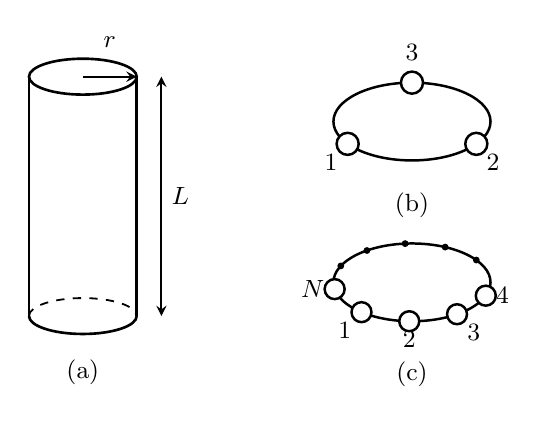
\begin{tikzpicture}[>=stealth, thick, scale=0.95]
  % Left: Smooth cylinder of radius r, length L (Fig 2)
  \begin{scope}[xshift=-3.0cm]
    \draw[line width=0.95pt] (0, 1.6) ellipse (0.72 and 0.24);
    \draw[line width=0.95pt] (-0.72, 1.6) -- (-0.72, -1.6);
    \draw[line width=0.95pt] (0.72, 1.6) -- (0.72, -1.6);
    \draw[line width=0.95pt] (-0.72, -1.6) arc (180:360:0.72 and 0.24);
    \draw[dashed, line width=0.65pt] (-0.72, -1.6) arc (180:0:0.72 and 0.24);
    % radius r
    \draw[->, line width=0.65pt] (0, 1.6) -- (0.72, 1.6);
    \node[above, font=\small] at (0.36, 1.85) {$r$};
    % length L
    \draw[<->, line width=0.65pt] (1.05, -1.6) -- (1.05, 1.6) node[midway, right, font=\small] {$L$};
    \node[below, font=\small] at (0, -2.05) {(a)};
  \end{scope}

  % Top-right: 3-atom ring (Fig 3)
  \begin{scope}[xshift=1.4cm, yshift=1.0cm]
    \draw[line width=0.9pt] (0, 0) ellipse (1.05 and 0.52);
    % Atoms 1, 2, 3
    \foreach \ang/\lbl/\pos in {215/1/below left, 325/2/below right} {
      \coordinate (p\lbl) at ({1.05*cos(\ang)}, {0.52*sin(\ang)});
      \fill[white] (p\lbl) circle (4.2pt);
      \draw[line width=0.9pt] (p\lbl) circle (4.2pt);
      \node[\pos, font=\small] at (p\lbl) {$\lbl$};
    }
    \fill[white] (0, 0.52) circle (4.2pt);
    \draw[line width=0.9pt] (0, 0.52) circle (4.2pt);
    \node[above, font=\small] at (0, 0.68) {$3$};
    \node[below, font=\small] at (0, -0.82) {(b)};
  \end{scope}

  % Bottom-right: N-atom ring (Fig 4)
  \begin{scope}[xshift=1.4cm, yshift=-1.15cm]
    \draw[line width=0.9pt] (0, 0) ellipse (1.05 and 0.52);
    \foreach \ang/\lbl/\pos in {190/N/left, 230/1/below left, 268/2/below, 305/3/below right, 340/4/right} {
      \coordinate (q\lbl) at ({1.05*cos(\ang)}, {0.52*sin(\ang)});
      \fill[white] (q\lbl) circle (3.8pt);
      \draw[line width=0.9pt] (q\lbl) circle (3.8pt);
      \node[\pos, font=\small] at (q\lbl) {$\lbl$};
    }
    % Dots along upper arc
    \foreach \ang in {35, 65, 95, 125, 155} {
      \fill ({1.05*cos(\ang)}, {0.52*sin(\ang)}) circle (1.3pt);
    }
    \node[below, font=\small] at (0, -0.92) {(c)};
  \end{scope}
\end{tikzpicture}
\end{document}
